\documentclass[
	paper=a4,				% set din paper format
	parskip=half,			% vertically separate paragraphs
	bibliography=totoc,     % literature in table of contents
	captions=tableheading,  % table heading
	titlepage=firstiscover, % titlepage is cover
]{scrartcl}

% improve float package
\usepackage{scrhack}
% center overwide objects
\usepackage{adjustbox}

% warn if recompile is necessary
\usepackage[aux]{rerunfilecheck}

% essential math commands
\usepackage{amsmath}
% many math symbols
\usepackage{amssymb}
% extensions for amsmath
\usepackage{mathtools}

% font settings
\usepackage{fontspec} % loads Latin Modern Fonts automatically, alternatives: Libertinus Serif/Sans/Mono

% recalculate page layout after setting differing fonts
\recalctypearea{}

% german language settings
\usepackage[ngerman]{babel}


\usepackage[
	math-style=ISO,		% ┐
 	bold-style=ISO,		% │
	sans-style=italic,	% │ follow iso standard
	nabla=upright,		% │
	partial=upright,	% ┘
	warnings-off={				% ┐
		mathtools-colon,		% │ remove redundant warnings
		mathtools-overbracket,	% ┘
	},
]{unicode-math}

% traditional math fonts
\setmathfont{Latin Modern Math} % alternative: Libertinus Math
\setmathfont[range=\mathbb]{texgyrepagella-math.otf}
% \setmathfont{XITS Math}[range={scr, bfscr}]
% \setmathfont{XITS Math}[range={cal, bfcal}, StylisticSet=1]

% numbers and units num, unit, qty, ang
\usepackage[
	locale=DE,						% german settings
	separate-uncertainty=true,		% always use pm for uncertainties
	per-mode=reciprocal,			% always use negative exponent
%	per-mode=symbol-or-fraction,	% symbol in inline math, fraction in display math
]{siunitx}

% chemical formulas
\usepackage[
	version=4,
	math-greek=default,	% ┐ allow functioning with unicode-math
	text-greek=default,	% ┘
]{mhchem}

% corrected quotation marks
\usepackage[autostyle]{csquotes}

% additional fraction type sfrac to frac, dfrac, tfrac, cfrac
\usepackage{xfrac}

% default placement for floats here, top, bottom
\usepackage{float}
\floatplacement{figure}{htbp}
\floatplacement{table}{htbp}

% control float behaviour
\usepackage[
	section,	% force floats to remain inside section
	below,		% allow placement below section on same page
]{placeins}

% rotate pages to landscape orientation for wide tables
\usepackage{pdflscape}

% improved captions
\usepackage[
	labelfont=bf,			% produce bold label in caption
	font=small,				% reduced fontsize relative to document
	width=0.9\textwidth,	% reduced caption width
]{caption}
% subfigure, subtable, subref
\usepackage{subcaption}

% include graphics
\usepackage{graphicx}

% draw pgf illustrations
\usepackage{tikz}
% draw pgf circuits
\usepackage[european]{circuitikz}

% create tables
\usepackage{booktabs}
\usepackage{multirow}

% edit enumeration parameters
\usepackage{enumitem}

% improved typeface
\usepackage{microtype}

% bibliography
\usepackage[
	backend=biber,
]{biblatex}
% source database
\addbibresource{lit.bib}
\addbibresource{programme.bib}

% hyperlinks inside document hyperref, href, eqref, ref
\usepackage[
	german,
	unicode,        % allow unicode in pdf attributes
	pdfusetitle,    % title, author, date as pdf attributes
	pdfcreator={},	% ┐ clean up pdf attributes
	pdfproducer={},	% ┘
	hidelinks,		% hide boxes around links
]{hyperref}
% extended bookmarks inside pdf
\usepackage{bookmark}

% separate words with hyphen
\usepackage[shortcuts]{extdash}

% increase bracket size for nesting
\delimitershortfall=-1pt

% input useful macros
% Hammerite, https://tex.stackexchange.com/a/257122

\usepackage{pgfmath, xparse}

\newlength{\MathStrutDepth}
\newlength{\MathStrutHeight}
\settoheight{\MathStrutHeight}{$\mathstrut$}
\settodepth{\MathStrutDepth}{$\mathstrut$}

\newlength{\NumeratorDepth}
\newlength{\DenominatorHeight}
\newlength{\DepthNegativeDifference}
\newlength{\HeightPositiveDifference}
\newlength{\NumeratorBaselineCorrection}
\newlength{\DenominatorBaselineCorrection}

\newlength{\AdditionalEVSFracVerticalSpacing}
\setlength{\AdditionalEVSFracVerticalSpacing}{0.05mm}

% Fraction with equal top-and-bottom vertical spacing around the bar.
% Suited only to simple fractions that do not appear near other fractions.
% When used alongside other fractions, numerator and denominator baselines
% might not be aligned, which might give ugly results.
% Additionally, the default line thickness for overlines and fractions is restored.
\NewDocumentCommand\pfrac{omom}{%
% 		\Umathfractionrule\displaystyle=0.4pt\relax
% 		\Umathoverbarrule\displaystyle=0.4pt\relax
% 		\Umathoverbarvgap\displaystyle=1.4pt\relax
% 		\Umathfractionrule\textstyle=0.4pt\relax
% 		\Umathoverbarrule\textstyle=0.4pt\relax
% 		\Umathoverbarvgap\textstyle=1.4pt\relax
% 		\Umathfractionrule\crampeddisplaystyle=0.4pt\relax
% 		\Umathoverbarrule\crampeddisplaystyle=0.4pt\relax
% 		\Umathoverbarvgap\crampeddisplaystyle=1.4pt\relax
% 		\Umathfractionrule\crampedtextstyle=0.4pt\relax
% 		\Umathoverbarrule\crampedtextstyle=0.4pt\relax
% 		\Umathoverbarvgap\crampedtextstyle=1.4pt\relax
    \IfValueTF{#1}%
              {\settodepth{\NumeratorDepth}{$#1$}}%
              {\settodepth{\NumeratorDepth}{$#2$}}%
    \IfValueTF{#3}%
              {\settoheight{\DenominatorHeight}{$#3$}}%
              {\settoheight{\DenominatorHeight}{$#4$}}%
    \pgfmathsetlength%
        {\DepthNegativeDifference}%
        {\NumeratorDepth - \MathStrutDepth}%
    \pgfmathsetlength%
        {\HeightPositiveDifference}%
        {\MathStrutHeight - \DenominatorHeight}%
    \pgfmathsetlength%
        {\NumeratorBaselineCorrection}%
        {\AdditionalEVSFracVerticalSpacing + \DepthNegativeDifference + \HeightPositiveDifference}%
    \pgfmathsetlength%
        {\DenominatorBaselineCorrection}%
        {-\AdditionalEVSFracVerticalSpacing}%
    \def\Numerator{\raisebox{\NumeratorBaselineCorrection}{$#2$}}%
    \def\Denominator{\raisebox{\DenominatorBaselineCorrection}{$#4$}}%
    \frac{\Numerator}{\Denominator}%
}
 % fraction type with equal v and h spacing pfrac

% tighter dotting in table of contents
\makeatletter
	\renewcommand\@dotsep{2}
	\renewcommand\@pnumwidth{0.75em}
\makeatother

% shortened commands
\def\bm{\symbf}

\author{
	Fritz Agildere\\ % Name
	\href{mailto:fritz.agildere@udo.edu}{fritz.agildere@udo.edu} % Email
	\and
	Amelie Strathmann\\ % Name
	\href{mailto:amelie.strathmann@udo.edu}{amelie.strathmann@udo.edu} % Email
}
\publishers{TU Dortmund – Fakultät Physik}



\subject{\texorpdfstring{\vspace{2ex}}{}V46\texorpdfstring{\vspace{-2ex}}{}} % Nummer
\title{Der Faraday-Effekt} % Titel: Name des Versuchs
\date{
	Durchführung: 15. April 2024 % Datum
	\\ Abgabe: 15. April 2024 % Datum
}

\begin{document}

\pagenumbering{gobble}

\maketitle
\thispagestyle{empty}

\pagenumbering{arabic}

\tableofcontents
\newpage

\section{Zielsetzung}
\label{sec:zielsetzung}

% Theorie: Physikalische Grundlagen von Versuch/Messverfahren, Gleichungen ohne Herleitung knapp erklären
\section{Theorie}
\label{sec:theorie}

Der Satz des Pythagoras beschreibt Seitenverhältnisse.

\subsection{Allgemein}

Für jedes rechtwinklige Dreieck kann
\begin{align}
	\label{eqn:allgemein}
	\stepcounter{equation}
	a^2 + b^2 &= c^2 \tag{1a} \\
	a^2 &= c^2 - b^2 \tag{1b}
\end{align}
geschrieben werden.

\subsection{Speziell}

Mit $a = b$ kann aus dem allgemeinen Fall \eqref{eqn:allgemein} direkt auf
\begin{equation}
	\label{eqn:speziell}
	2a^2 = c^2
\end{equation}
geschlossen werden.

\section{Aufbau}
\label{sec:Aufbau}


% Vorbereitung: Vorbereitungsaufgaben bearbeiten
% Versuchsaufbau: Verwendete Apparatur, Beschreibung Funktionsweise/Nutzen mit Skizze/Foto
\section{Durchführung}
\label{sec:durchführung}

\section{Auswertung}
\label{sec:auswertung}

Im Folgenden werden die aufgenommenen Messdaten ausgewertet, um den Kernspin der Isotope zu bestimmen.
Dafür müssen zunächst die Landé-Faktoren der Isotope bestimmt werden und die vertikale Komponente des Erdmagnetfeldes.
Anschließend wird das Isotopenverhältnis der Rubidium-Isotope bestimmt und der quadratische Zeeman-Effekt untersucht.

Es werden die Werte der Magnetfeldstärken der Horizontalen Spule berechnet, indem die jeweiligen Anteile der Sweep und der
horizontalen Verschiebungsspule addiert werden.
Für die Magnetfeldstärken der Spulen im Zentrum gilt

\begin{equation}
    B(0) = \frac{8  \mu_0  N I}{\sqrt{125} A}  \, .
    \label{eqn:magnetfeld}
\end{equation}

Die Stromstärke des Sweepanteils wird per Umdrehung gemessen.
Dieser Wert wird mit \qty{0.1}{\ampere} pro Umdrehung umgerechnet.
Für den horizontalen Anteil wurde die Spannung in \unit{\milli\volt} gemessen und kann umgerechnet werden in \unit{\milli\ampere},
indem die Werte der Spannungen verdoppelt werden.
Die notierten Werte werden in Tabelle \ref{tab:magnetfeldstärken} aufgetragen, wobei die Stromstärken bereits umgerechnet wurden.

\begin{table}
    \centering
    \caption{Die aufgenommenen Messwerte der Sweep-Spule und der horizontalen Verschiebungsspule für beide Isotope.}
    \label{tab:magnetfeldstärken}
    \begin{tabular}{c c c c c}
        \toprule
        $f \mathbin{/} \mathrm{kHz} $& $I_{S1} \mathbin{/} \unit{\ampere}$ & $I_{H1} \mathbin{/} \unit{\ampere}$ & $I_{S2} \mathbin{/} \unit{\ampere}$ & $I_{H2} \mathbin{/} \unit{\ampere}$ \\
        \midrule
        100 & 0.54 & 0.00 & 0.658 & 0.00 \\
        200 & 0.776 & 0.00 & 0.731 & 0.0194 \\
        300 & 0.436 & 0.0402 & 0.790 & 0.0402 \\
        400 & 0.328 & 0.0642 & 0.801 & 0.0642 \\
        500 & 0.291 & 0.0834 & 0.891 & 0.0834 \\
        600 & 0.281 & 0.1006 & 0.987 & 0.1006 \\
        700 & 0.10 & 0.1298 & 0.928 & 0.1298 \\
        800 & 0.272 & 0.1374 & 0.433 & 0.1894 \\
        900 & 0.384 & 0.1432 & 0.598 & 0.2028 \\
        1000 & 0.459 & 0.2374 & 0.522 & 0.2328 \\
        \bottomrule
    \end{tabular}
\end{table}

In Abbildung \ref{fig:plot1} sind die mit der Gleichung \ref{eqn:magnetfeld} berechneten Magnetfeldstärken gegen die Frequenz für beide Isotope aufgetragen.

\begin{figure}
    \centering
    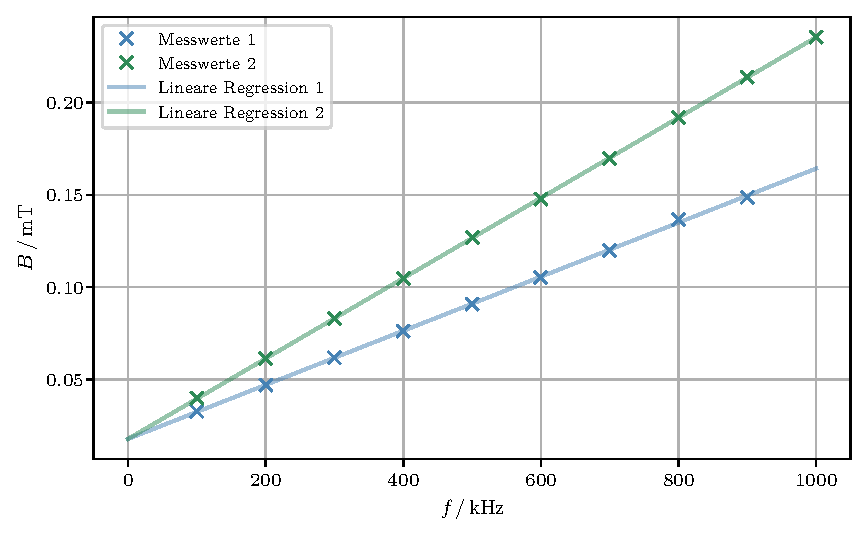
\includegraphics[width=0.8\textwidth]{build/plot.pdf}
    \caption{Magnetfeldstärke aufgetragen gegen die Frequenz für beide Isotope.}
    \label{fig:plot1}
\end{figure}

Es wurde eine lineare Regression der Messwerte für beide Isotope durchgeführt.
Während der Ausgleichsrechnung ist aufgefallen, dass bei dem letzten Wert der erste Peak zweimal vermessen wurde.
Daher wird dieser Messwert für den zweiten Peak bei der weiteren Berechnung vernachlässigt.
Die verwendete Ausgleichsfunktion hat die Form
\begin{equation}
    f(x) = a \cdot x + b \, .
\end{equation}

Daraus folgen die Parameter beider Isotope
%a_1: (1.468+/-0.011)e-07
%b_1: (1.76+/-0.06)e-05
%a_2: (2.1795+/-0.0035)e-07
%b_2: (1.760+/-0.022)e-05

\begin{align*}
    a_1 &= \qty{1.468(11)e-07}{\tesla\per\hertz} \\
    b_1 &= \qty{1.76(6)e-05}{\tesla} \\
    a_2 &= \qty{2.1795(35)e-07}{\tesla\per\hertz} \\
    b_2 &= \qty{1.760(22)e-05}{\tesla} \, .
\end{align*}

Die berechneten Werte werden für die weiteren Rechnungen verwendet.

\subsection{Magnetfeld der Erde}
\label{sec:magnetfeld-der-erde}

Die Vertikalkomponente des Erdmagnetfeldes hat aufgrund des horizontal verlaufenden Lichtstrahls einen Einfluss auf die Messung.
Daher wird diese durch ein vertikal verlaufendes Magnetfeld kompensiert und der Aufbau wird um die vertikale Achse in Nord-Süd Richtung gedreht,
sodass die horizontale Komponente parallel oder antiparallel zu dem horizontalen Magnetfeld verläuft.
Zur Berechnung der Feldstärke des Erdmagnetfeldes muss zunächst die magnetische Feldstärke des vertikalen Feldes gemessen werden.
Diese betrug in diesem Experiment \qty{0.23}{\ampere}.

Anschließend wird über den $y$-Achsenabschnitt der Ausgleichsgeraden in Abbildung \ref{fig:plot1} die horizontale Magnetfeldstärke bestimmt.
Der Mittelwert der $y$-Achsenabschnitte wird mittels uncertainties \cite{uncertainties} gebildet, um den Wert des horizontalen Feldes zu bestimmen.
Über den Satz des Pythagoras kann der Wert des Erdmagnetfeldes ermittelt werden.
Schlussendlich ergibt sich für das Magnetfeld der Erde \qty{3.939(15)e-05}{\tesla}.

\subsection{Bestimmung Landé-Faktor}
\label{sec:best-lande-faktoren}

Durch Umstellen der Gleichung \ref{eqn:larmor} kann auf den Zusammenhang
\begin{equation}
    g_{\text{F}} = \frac{h}{\mu_B a }
\end{equation}
geschlossen werden.
Für die Landé Faktoren der Isotope ergeben sich die Werte
\begin{align}
    g_1 &= \num{0.487 +- 0.004} \\
    g_2 &= \num{0.328 +- 0.001} .
\end{align}

Anhand der in Abschnitt \ref{sec:theorie} theoretisch bestimmten Werte für die Landé Faktoren der beiden Isotope (Rb-85 \ref{eqn:vorhesage_85} und Rb-87 \ref{eqn:vorhesage_87}) können schließlich
die experimentellen Werte zugeordnet werden.
Daher enspricht $g_1$ dem Wert des Isotops Rb-87 und $g_2$ kann zu dem Isotop Rb-85 zugeordnet werden.
Im Folgenden werden auch die jeweiligen Ausgleichsgeraden zugeordnet.
Die lineare Regression 1 entspricht daher Rb-87 und die lineare Regression 2 gehört zu Rb-85.

\subsection{Kernspin der Rubidium-Isotope}
\label{sec:Kernspin der Rubidium-Isotope}

Mittels der bestimmten $g_{\text{F}}$-Faktoren kann anschließend der Kernspin berechnet werden.
Aus der Formel \ref{eqn:lande_J} und den Werten der Quantenzahlen, welche in Abschnitt \ref{sec:theorie} angegeben sind,
ergibt sich $g_{\text{J}} = 2$.
Somit sind alle benötigten Variablen bekannt.

Der Kernspin der Isotope kann durch Umstellen der Gleichung \ref{eqn:lande_F} berechnet werden.
Es folgt für den Kernspin
\begin{equation}
    I = -\frac{1}{2} + \sqrt{1 + F(F+1) \cdot (1 - g_{\text{F}})} \, .
\end{equation}

Für die Isotope Rb-85 und Rb-87 ergeben sich die experimentell bestimmten Kernspins
\begin{align}
    I_{85} &= \num{2.511(1)} \\
    I_{87} &= \num{1.520(5)} \, .
\end{align}

\subsection{Isotopenverhältnis}
\label{sec:Isotopenverhältnis}

Wegen besserer Ablesbarkeit der Peaks wird die Aufnahme des Oszilloskops bearbeitet, diese ist in Abbildung \ref{fig:edit} zu sehen.

\begin{figure}
    \centering
    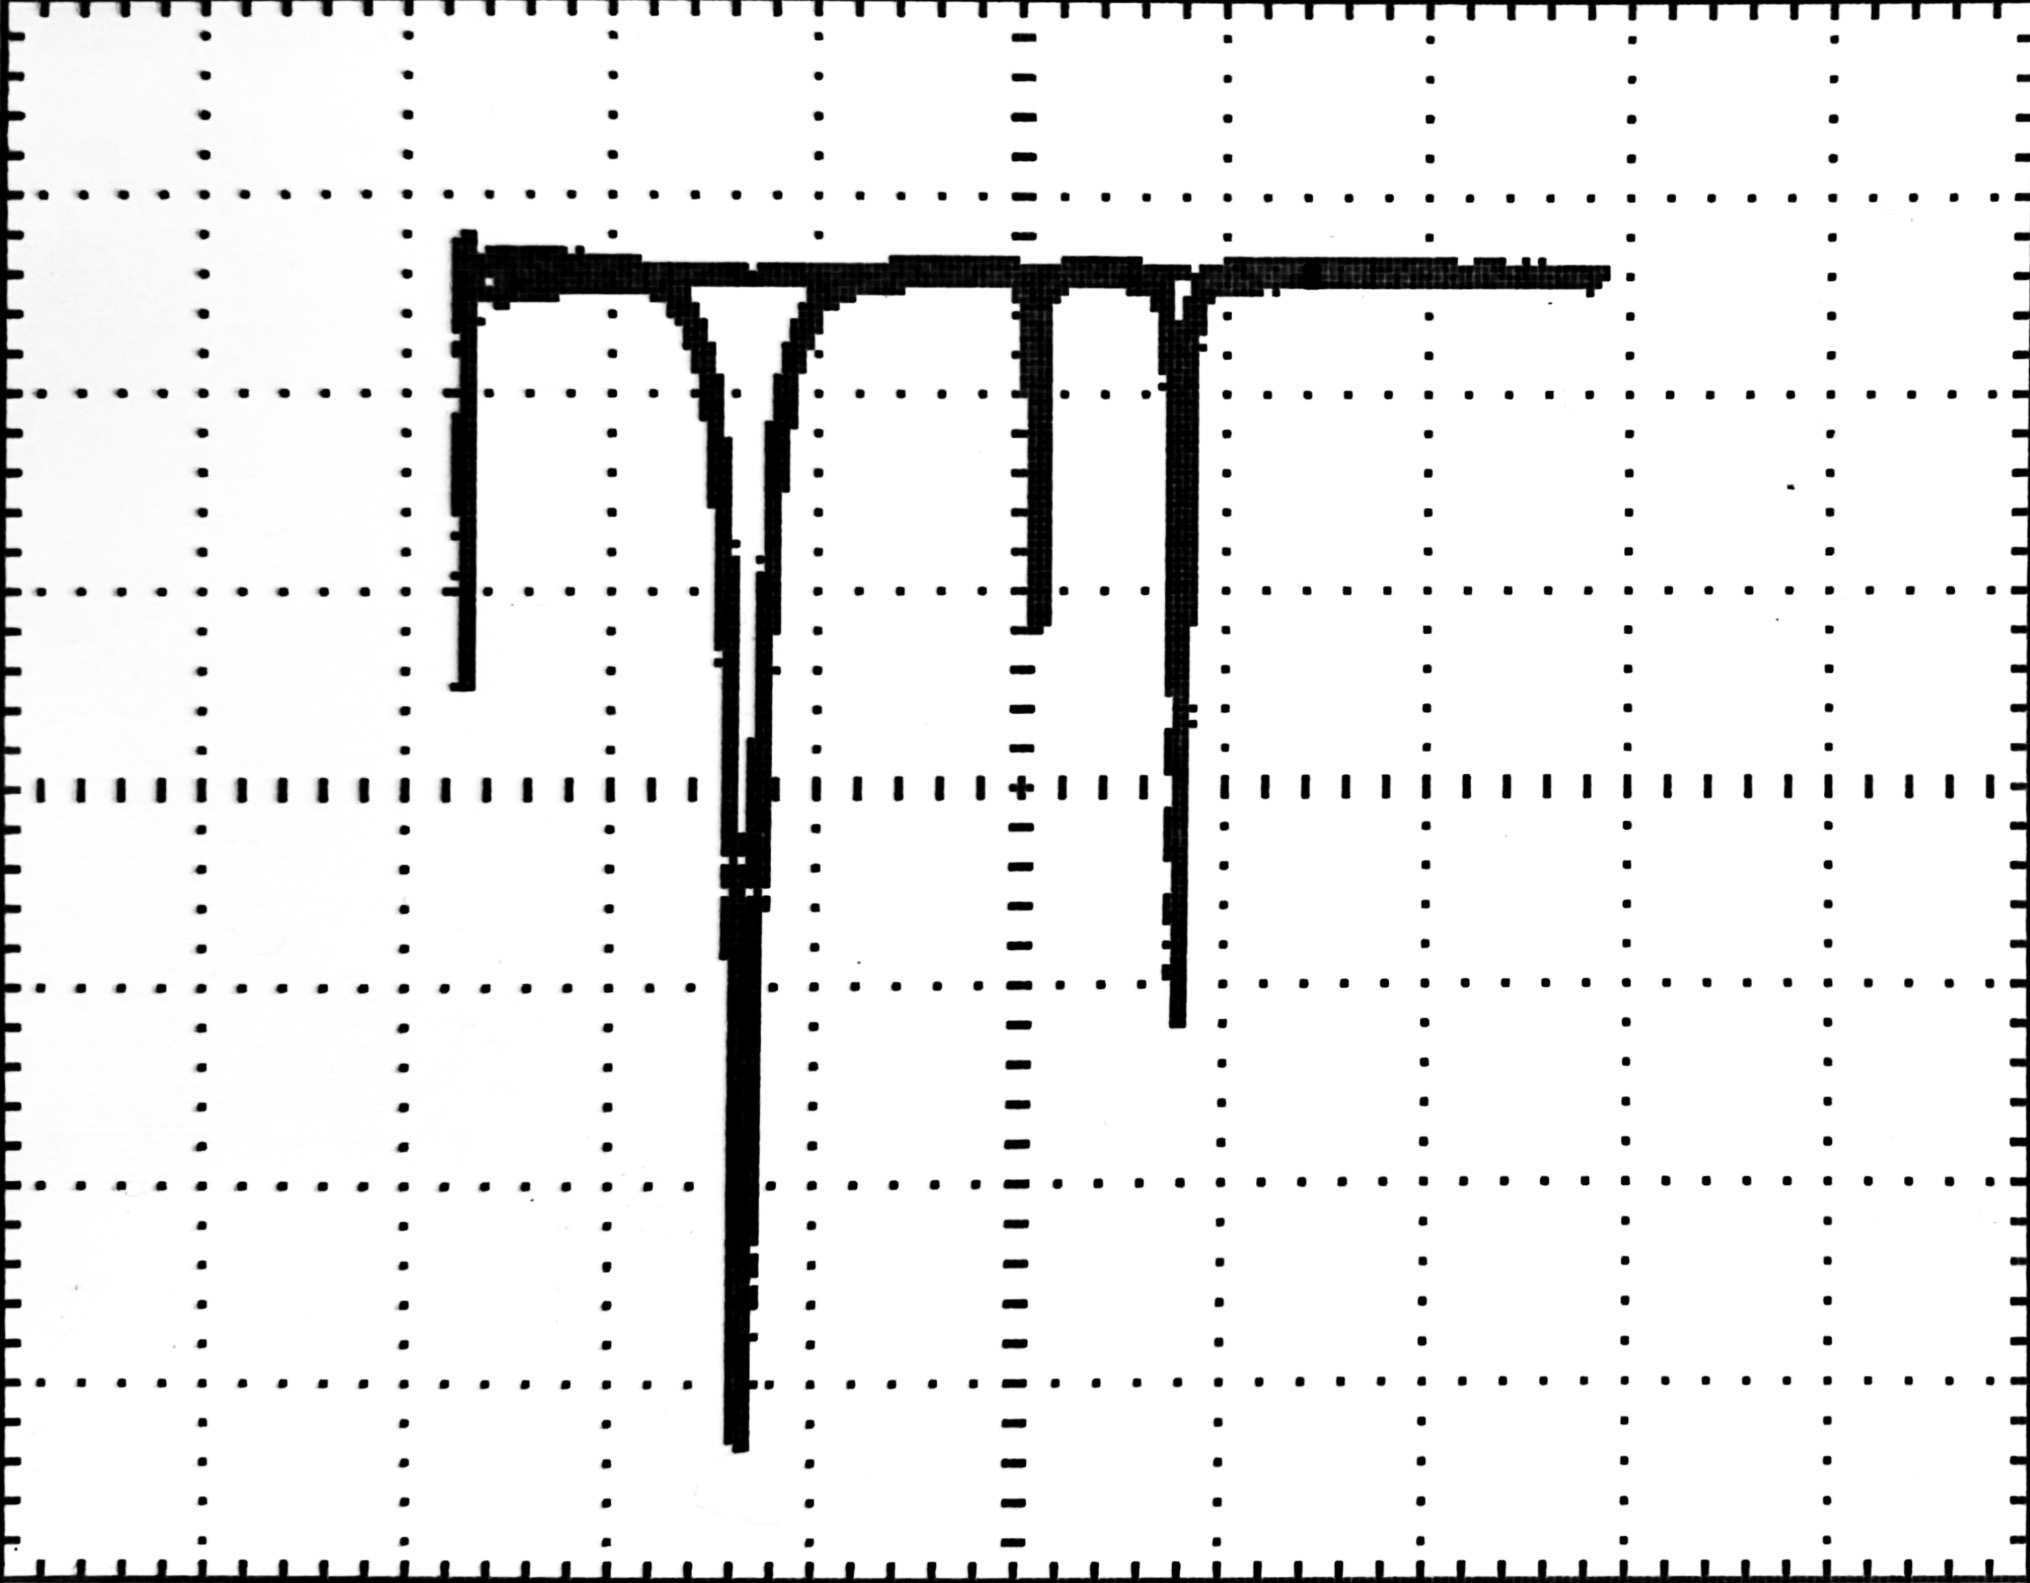
\includegraphics[width=0.6\textwidth]{content/messung/edit.jpg}
    \caption{Bearbeitete Aufnahme des Oszilloskops.}
    \label{fig:edit}
\end{figure}

Die Aufnahme der Resonanzstellen wurde bei einer Frequenz von $f = \qty{100}{\kilo\hertz}$ getätigt.
Um das Isotopenverhältnis zu bestimmen, werden die Amplituden der Resonanzstellen abgelesen, indem
die Kästchen auf dem Oszilloskop gezählt werden.
Der erste kleinere Peak gehört zu dem Isotop Rb-87 und der größere zu Rb-85.
Der erste Peak hat eine Tiefe von ungefähr 2 Kästchen und der zweite besitzt eine Tiefe von ungefähr 4 Kästchen.
Das Verhältnis ist daher 1:2.
Daraus folgt für die Anteile
\begin{align}
    P_1 &\approx 33 \% \\
    P_2 &\approx 67 \% .
\end{align}

\subsection{Quadratischer Zeeman-Effekt}
\label{sec:quadratischer-zeeman-effekt}

Zusammen mit der Gleichung \ref{eqn:quad_zeeman} und den Theoriewerten in der Tabelle \ref{tab:zee}, kann die
quadratische Zeeman-Aufspaltung berechnet werden.

\begin{table}
    \centering
    \caption{Theoriewerte der Isotope zur Berechnung der Zeemann Aufspaltung und experimentell bestimmte Werte des B-Feldes. \cite{pumpen}}
    \label{tab:zee}
    \begin{tabular}{c c}
        \toprule
        Rb-87 & Rb-85\\
        \midrule
        $B = \qty{0.0909}{\milli\tesla}$ & $B = \qty{0.137}{\milli\tesla}$ \\
        $M_f = 2$ & $M_f = 3$ \\
        $\Delta E_{hf} = \qty{4.53e-24}{\joule} $ & $\Delta E_{hf} = \qty{2.01e-24}{\joule} $ \\
        \bottomrule
    \end{tabular}
\end{table}

Somit ergeben sich die Werte der quadratischen Zeeman-Aufspaltung für beide Isotope
\begin{align}
    \Delta E_Z^{87} &= \qty{2.606(0.004)}{\nano\eV} \\
    \Delta E_Z^{85} &= \qty{2.562(0.019)}{\nano\eV} .
\end{align}

\section{Diskussion}
\label{sec:diskussion}

Während des Prozesses der Auswertung ist aufgefallen, dass anstelle des zweiten Peaks erneut der erste vermessen wurde.
Um die diese Fehlerquelle in der Ausgleichsrechnung zu eliminieren, wurden die Werte des Rb-85 Peaks entfernt.

Der theoretische Wert des Erdmagnetfeldes in NRW beträgt \qty{48}{\micro\tesla} (\cite{erdmagnetfeldstärke}).
Die experimentell bestimmte Magnetfeldstärke der Erde hat den Wert \qty{39.39(15)}{\micro\tesla}.
Der experimentelle Wert weicht um \num{17.94(0.31)} \% nach unten von dem theoretischen Wert ab.
Dieser Fehler liegt im akzeptablen Bereich, da während des Experimentes systematische aufgetreten sein können.
Zunächst kann die genaue örtliche Lage der Versuchsdurchführung einen Einfluss auf den Wert haben, weil
der Aufbau sich in einem Gebäude aus Beton und Stahl befindet.
Dies kann das $B$-Feld abschirmen.
Zudem musste der Versuchsaufbau in Nord-Süd Richtung justiert werden, dies wurde per Augenmaß abgeschätzt.
Durch Einstellung des vertikalen Magnetfeldes sollte der vertikale Teil des Erdmagnetfeldes kompensiert werden.
Infolgedessen wurde dieses vertikale $B$-Feld anhand des Oszillografen eingestellt und abgelesen.
Der horizontale Anteil des Erdmagnetfeldes wurde anhand einer Linearen Ausgleichsrechnung für jeweils beide Isotope bestimmt.
Anschließend wurde der Mittelwert beider Datenpunkte berechnet.
Daraus folgt ein statistischer Fehler, welcher das experimentelle Ergebnis beeinflussen kann.

Rb-87 hat in der Theorie einen Landé-Faktor von $g_F^{87} = 1/2$ und der Landé-Faktor des anderen Isotops besitzt den Wert $g_F^{85} = 1/3$.
Bei dem Versuch wurden die experimentellen Werte $g_{87} =$ \num{0.487 +- 0.004}  und $g_{85} = $  \num{0.328 +- 0.001} berechnet.
Das Ergebnis des Rb-87 Isotops weicht um \num{2.6(0.07)} \% nach unten ab und bei dem Rb-85 weicht der experimentelle Wert um \num{1.65(0.016)} \% nach unten ab.
Daher konnte der Landé-Faktor experimentell sehr annehmbar bestimmt werden.
Kleinere Abweichungen können aus den statistischen Fehlern folgen, die währende der Fehlerrechnung entstehen.
Außerdem wurden die einzelnen Peaks händisch vermessen, was ebenfalls zur Fehlerquelle werden kann.

Die theoretischen Werte des Kernspins der Isotope sind $I_{85} = 5/2$ und $I_{87} = 3/2$.
Die experimentell bestimmten Werte sind $I_{85} = \num{2.511(1)}$ und $I_{87} = \num{1.520(5)}$.
Der experimentelle Wert des Rb-85 Isotops weicht um \num{0.44(0.04)} \% nach oben ab und der Wert des Rb-87 Isotops weicht um \num{1.3(0.4)} \% nach oben ab.
Die Abweichungen sind sehr gering und liegen im akzeptablen Bereich.
Diese Unterschiede können durch die statistischen Fehler, die während der Fehlerrechnung entstehen, erklärt werden.
Zusätzlich sollten immer die systematischen Fehler beachtet werden, die während des Versuches auftreten können.

Das Isotopenverhältnis in dem vorliegenden Versuch beträgt 1:2, wobei Rb-85 das häufigere Isotop ist.
In der Natur beträgt der Anteil von Rb-87 27.83 \% und der Anteil von Rb-85 72.17 \% (\cite{rubidium}).
Es kann vermutet werden, dass Rb-87 in dem Versuch angereichert wurde, um den entsprechenden Peak besser sichtbar zu machen.

Abschließend werden die Größenordnungen der Zeeman-Aufspaltungen mit der Hyperfeinstruktur Aufspaltung verglichen.
Die Zeeman-Aufspaltungen liegen im Bereich \qty{\nano\eV}.
Die Hyperfeinstruktur Aufspaltung ist um vier Größenordnungen größer.

Insgesamt konnte die Auswertung des Versuches erfolgreich durchgeführt werden und die experimentellen Werte liegen im akzeptablen Bereich.


\enlargethispage{2\baselineskip}\printbibliography{}\pagebreak

\newpage
\section*{Anhang}

\addcontentsline{toc}{section}{Anhang}

\centering

\vfill

\includegraphics{content/messung/1.jpg}
\vfill


\end{document}
